This section describes the entire model formally using the alloy language. 
In particular, we aim to:
\begin{enumerate}
    \item model the interaction between students
          in order to create teams which can partecipate to battles
    \item model the interactions related to the creation and management
          of tournaments as well as battles, in order to prove that 
          authorization is represented properly by the model
\end{enumerate}

\subsection{Alloy Code}
\lstinputlisting[language=alloy]{alloy/model.als}

\pagebreak
\subsection{Models}

\begin{enumerate}[label=,leftmargin=0cm]
    \item \textbf{Team of students partecipate in a battle}
          
          This model was generated using:
          \begin{lstlisting}[language=alloy]
            run {
                #Battle = 1 
                some b: Battle | b.minStudents = 3 and 
                                b.maxStudents = 3 and 
                                #b.partecipations >= 1
                #Team = 2
                #Invite = 4
                some i: Invite | i.state = Rejected
                some i: Invite | i.state = Pending
                #Student = 4
                #Educator = 1
                #Badge = 0
            } for 10
          \end{lstlisting}
          
          \begin{adjustbox}{max size={\textwidth}{\textheight}}
              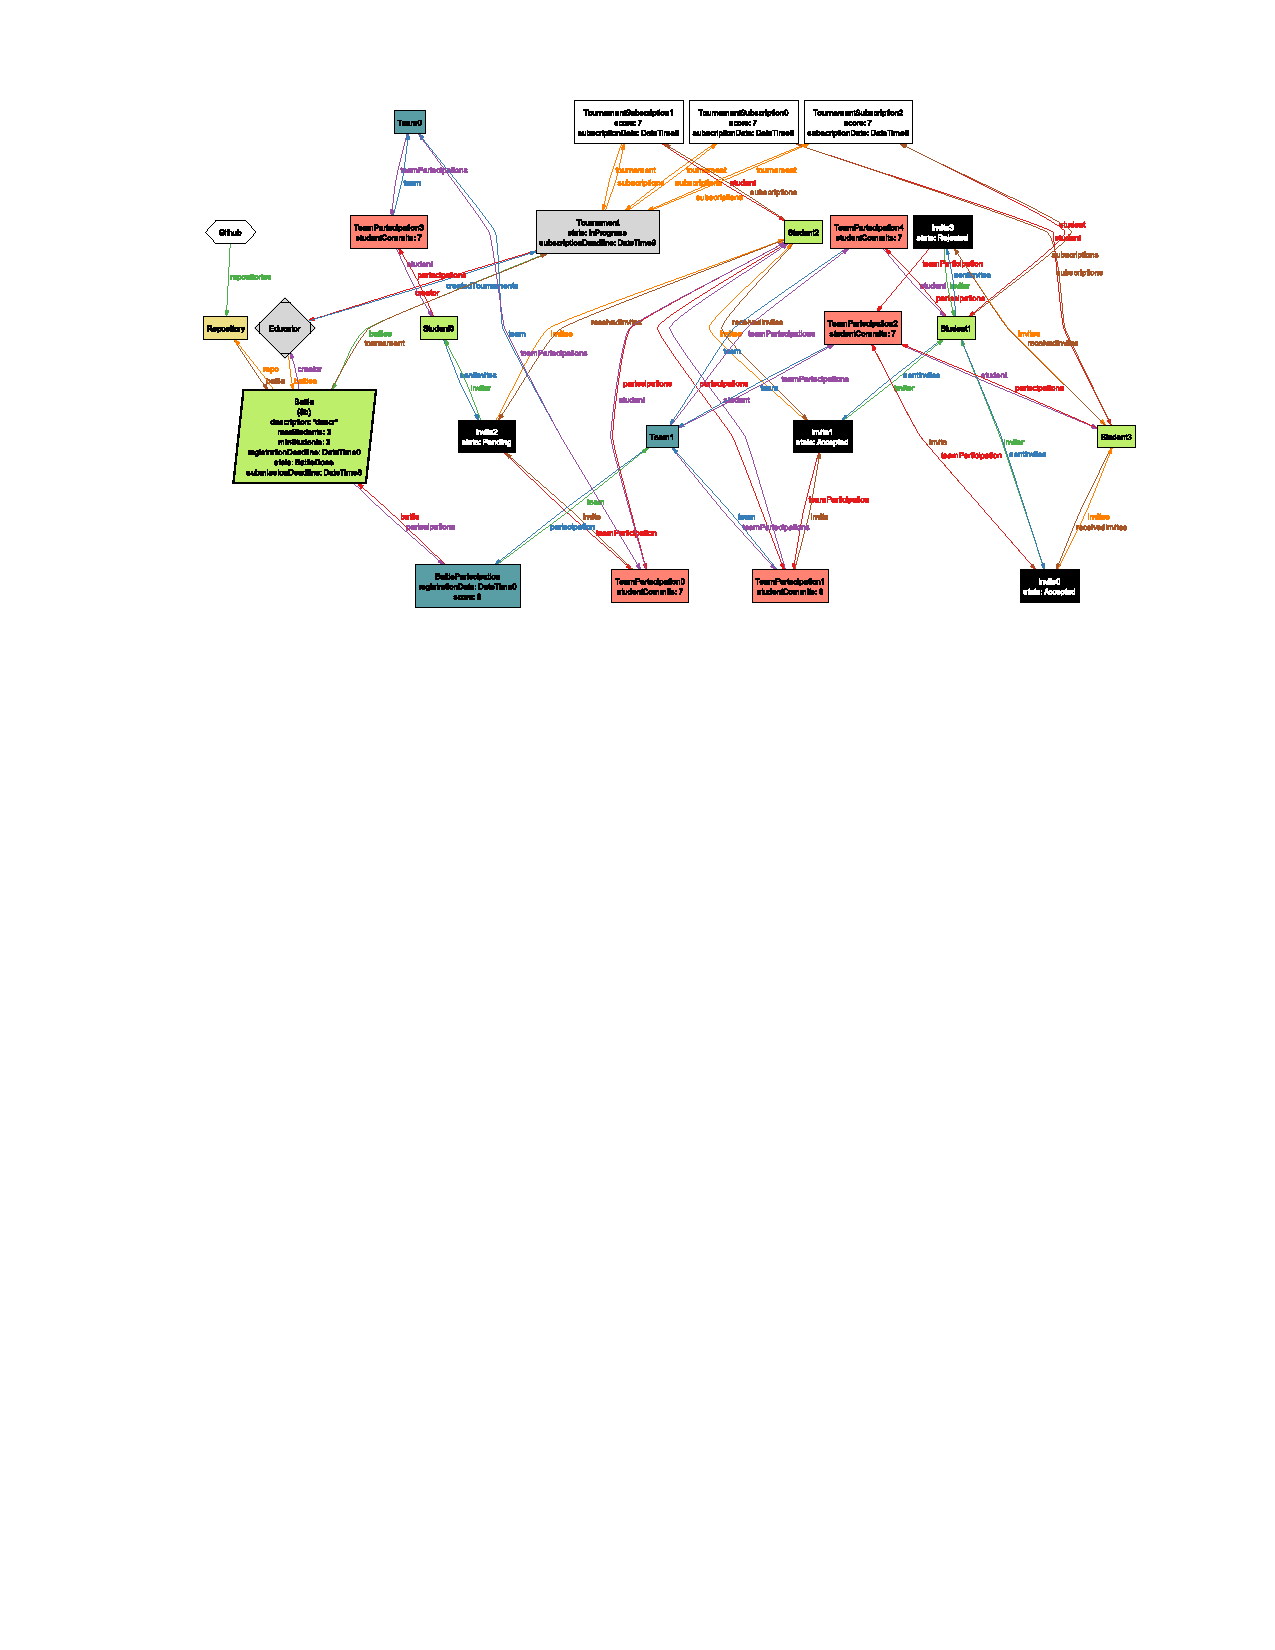
\includegraphics[trim=90 475 60 40, clip]{alloy/invites.pdf}
          \end{adjustbox}
          
          The diagram shows that:
          \begin{enumerate}
              \item only one student (the team creator) can send invites
                    to join the team (Student0 for Team0 and Student1 for Team1)
              \item if the team has already been subscribed to a battle
                    all the invites must have been accepted
              \item you can receive multiple invites to the same team only
                    if you rejected the previous ones (such as Student3)
              \item you can receive invites for multiple teams, given they are not
                    for the same battle (such as Student2)
          \end{enumerate}
          \pagebreak
    \item \textbf{Management of tournaments and battles}
          
          This model was generated using:
          \begin{lstlisting}[language=alloy]
            run {
                #Student = 0 
                #Tournament = 2
                #Battle >= 3
                #Educator >= 3
                #Badge >= 2
            } for 10
          \end{lstlisting}
          
          \begin{adjustbox}{max size={\textwidth}{\textheight}}
              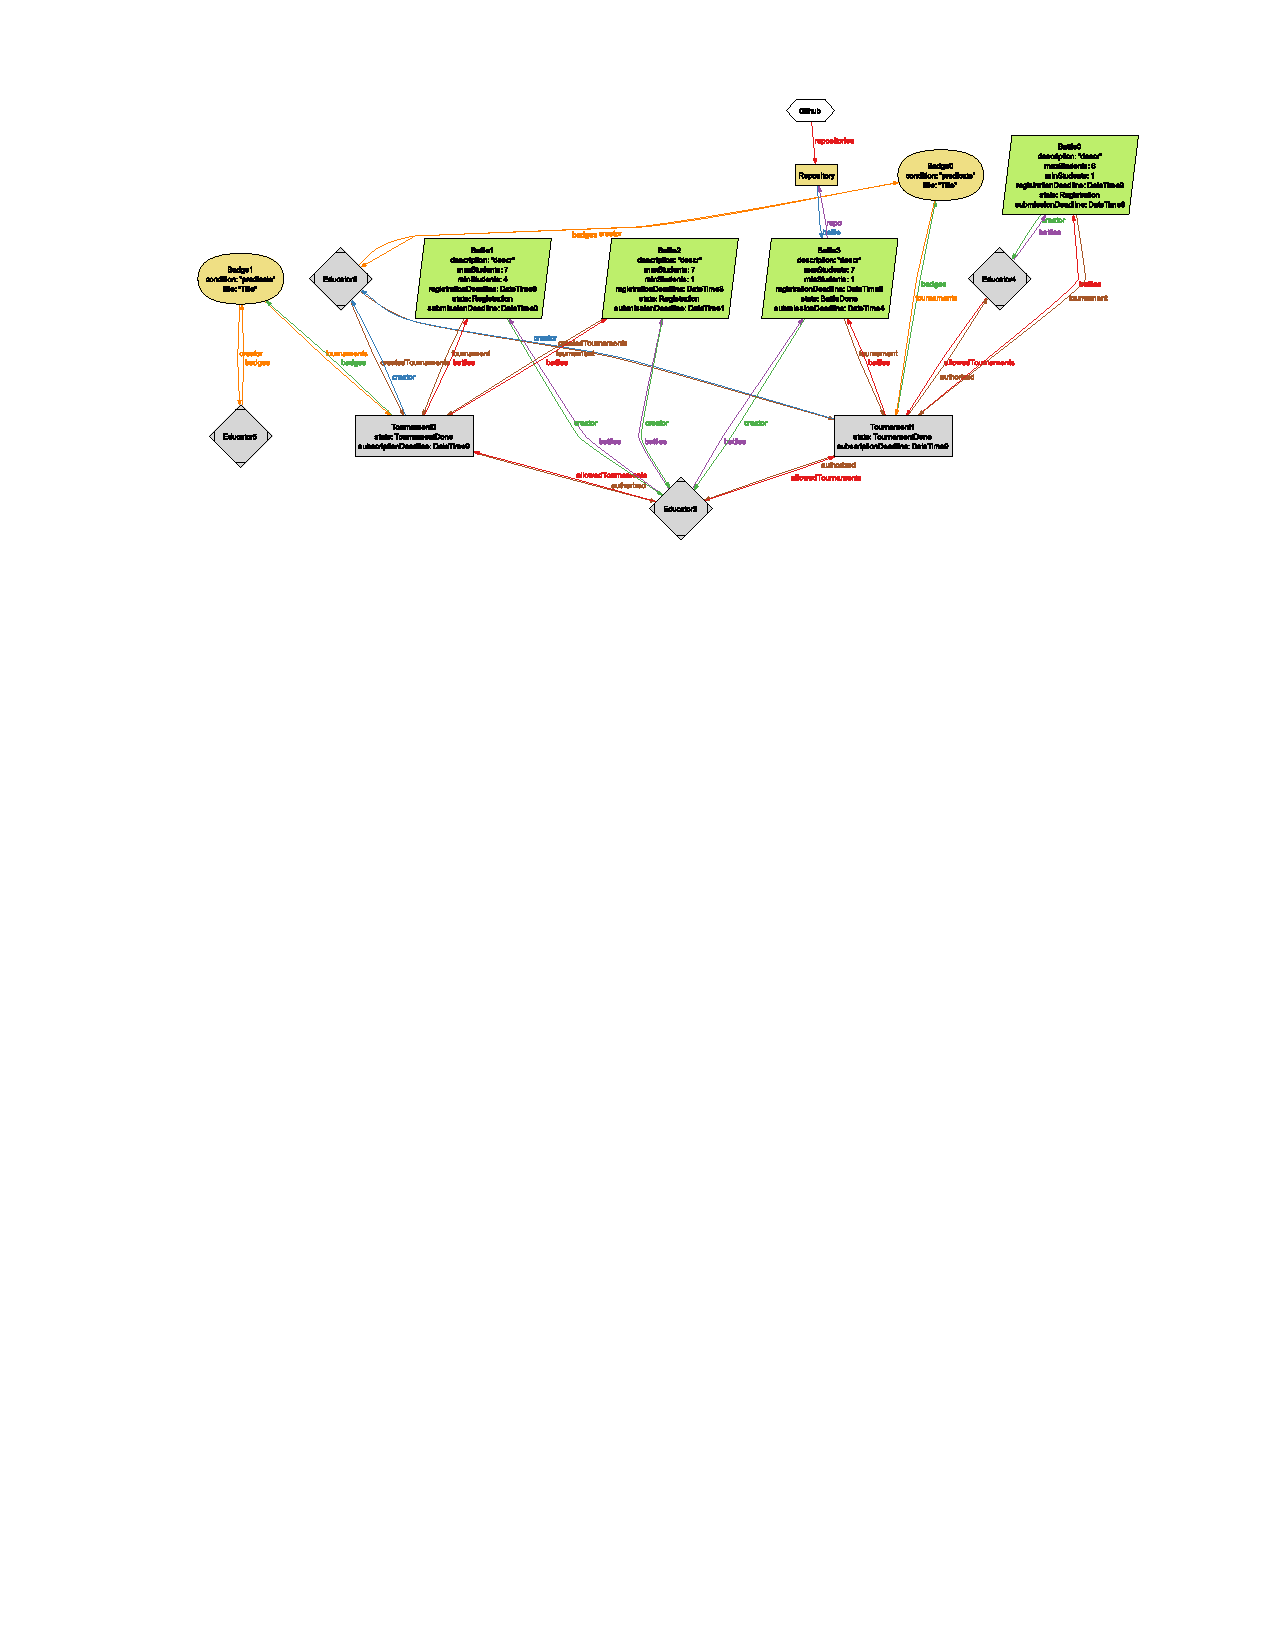
\includegraphics[trim=90 525 60 40, clip]{alloy/manage_tournaments.pdf}
          \end{adjustbox}
          
          The diagram shows that:
          \begin{enumerate}
              \item Educator3 has not created any tournament, yet they are authorized
                    to create battles in both and they have done so
              \item Educator4 has created a tournament and a corresponding battle in it
              \item Educator5 has created a badge unrelated to the tournaments shown here,
                    however it can be reused by other teachers
          \end{enumerate}
\end{enumerate}